\section{Transformers}

\subsection{Token Paradigm}
Given is a sequence of tokens in the form of their respective embeddings $X = \left[x_1, \dots, x_T\right]\in \mathbb{R}^{n\times T}$. The fundamental idea is to map the non-contextualized embeddings $X$ to contextualized representations $\Xi = \left[\zeta_1, \dots, \zeta_T\right]\in \mathbb{R}^{m \times T}$. 

\subsection{Attention Mixing}
An attention mechanism produces numbers $\alpha_{s, t}$ that are then used to convexly combine the input representations into new representations $\zeta_s = \Sigma_t \alpha_{s, t}Wx_t$, where $\alpha_{s, t} \geq 0$ and $\Sigma_t \alpha_{s, t} = 1$. 

\textbf{Remarks:}\begin{itemize}
    \item The attention weights $\alpha_{s, t}$ have a \textbf{source} (where attention emerges, $s$) and a \textbf{target} (where attention extracts information, $t$)
    \item In matrix notation, we write $A = (a_{st}) \in \mathbb{R}^{T \times T}$, such that $\Xi = WXA^{\intercal}$. 
    \item Attention mechanism mixes information across columns of $X$ via $A^{\intercal}$, and mixes dimensions linearly via $W$. 
\end{itemize}

\subsection{Query-Key Matching}
\textbf{Question:} How to learn $A$?
\begin{enumerate}
    \item Project $X$ to query matrix $Q = U_QX$ and key matrix $K=U_KX$, where $U_Q, U_K \in \mathbb{R}^{q \times n}$
    \item Produce matching matrix by matching keys and queries via inner products: $Q^{\intercal}K = X^{\intercal}U_Q^{\intercal}U_KX \in \mathbb{R}^{T \times T}$ (note that $rank(U_Q^{\intercal}U_K) \leq q$)
    \item Soft-max transformation: $A = \text{softmax}(\beta Q^{\intercal}K)$ where $a_{st} = \frac{e^{\beta[Q^{\intercal}K]_{st}}}{\Sigma_re^{\beta[Q^{\intercal}K]_{sr}}}$
\end{enumerate}

\textbf{Inverse temperature $\beta$:} Controls the entropy of the softmax and is not learned, but usually chosen as $\beta = 1/\sqrt{q}$ (to standardize the size of $Q^{\intercal}K$ dot products to be independent of $q$). \textbf{Higher} $\beta$ leads to \textbf{lower entropy} of the softmax and the \textbf{attention} becomes \textbf{more selective/focused} on the highest-scoring queries/keys (and vice-versa for lower $\beta$)


\subsection{Multi-Headed Attention}
\textbf{Idea:} Run multiple attention models in parallel. 
\begin{itemize}
    \item Replicate the matrices $U_K, U_Q, W$ a total of $r$ times
    \item Perform attention-based propagation $X \mapsto \Xi_i$ for $i = 1, \dots, r$
    \item Concatenate the matrices $\Xi_i$ along the feature dimension
\end{itemize}
Concrete numbers from \textit{Attention Is All You Need} are: feature space dimension $n = 512$, number of heads $r = 8$, query/key space dimension $q = 64$. 


\textbf{Remark:} Originally proposed values for $r, q$ and $n$ ensure that after concatinating the different heads, the output dimension stays the same ($8 \cdot 64=512$). The reasons for this \textit{trick}: 
\begin{itemize}
    \item Residual connections: Would not be possible with different dimensions.
    \item Efficiency costs: Less parameters to estimate.
    \item Scalability: The output dimension would increase with every layer by a factor of $r$, if we would not use this trick.
\end{itemize}


\subsection{Feature Transformation}
\textbf{Issue:} Attention mechanism \textbf{only} performs convex combination of columns of $X$, which is insufficient (even if the relative weights are non-linear functions of $X$). 


\textbf{Solution:} Gain representational power by \textbf{applying a per-token} transformation with a feedforward network. Formally, $X \mapsto \Xi \mapsto F(\Xi)$, where $F(\Xi) = (F(\zeta_1), \dots, F(\zeta_T))$ operates on the columns of $\Xi$. 


\subsection{Positional Encoding}
\textbf{Issue:} Attention mechanism operates on (unordered) set of tokens ($\leadsto \text{value of token position is lost}$)


\textbf{Solution:} Assign each non-negative integer $t$ to a low-dimensional vector and add this vector to the respective token embedding $x_t$. 


\textbf{Sinusoidal Encoding:} $p_{tk} = \begin{cases}
    sin(t\omega_k) \quad k \text{ even}\\
    cos(t\omega_k) \quad k \text{ odd}
\end{cases}$, where $\omega_k = C^{n/k}$ and $n$ is the feature space dimension ($=512$ in the original paper)


\subsection{Masked and Cross-Attention}
\textbf{Masked Attention:} In cases where transformers operate in coupled encoder-decoder pairs, the decoder typically operates in autoregressive fashion (output at $t$ depends on encoder, but also on produced token representations for $s < t$). Masked attention restricts the attention to the past. 
\textbf{Cross-Attention: } Attention to representations produced by the encoder. Cross-Attention is implemented across layers of the same depth. Note that in cross-attention the queries emerge from the decoder, whereas the keys and values are derived from the encoder states. 

\subsection{Transformer} \vspace{-0.18cm}
\begin{center}
    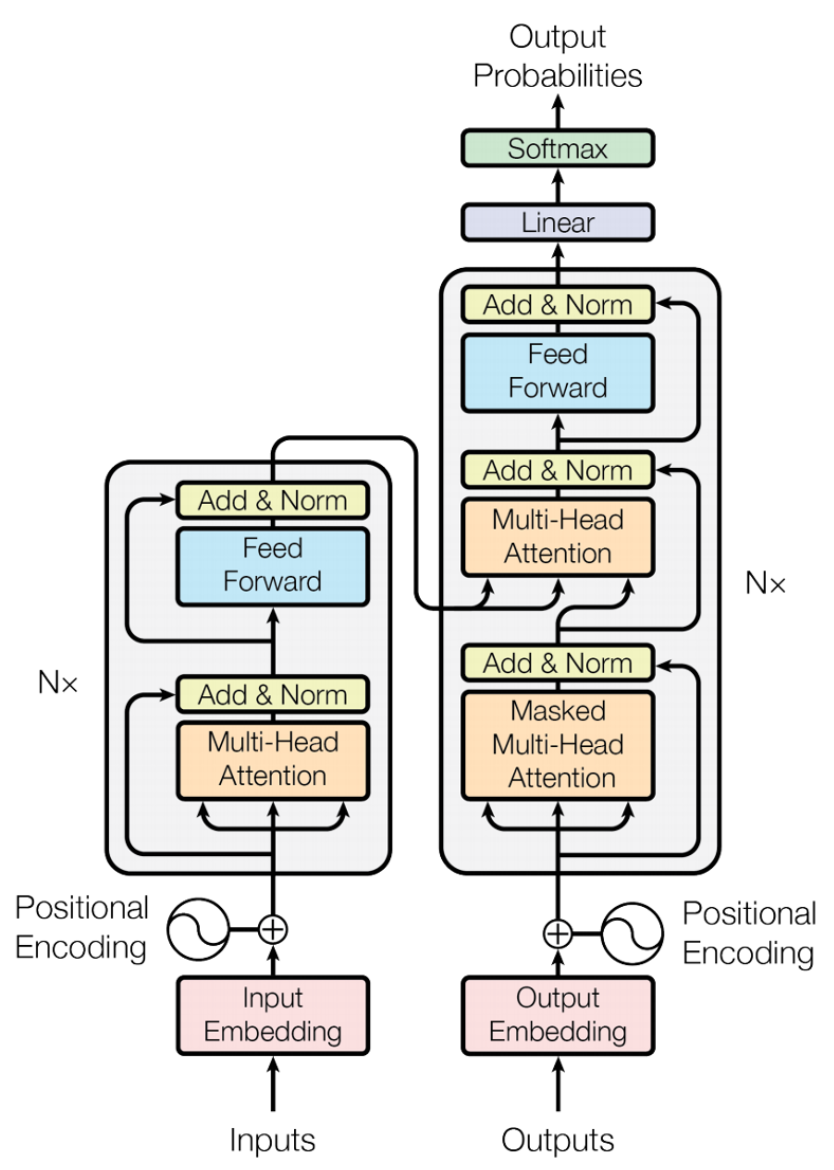
\includegraphics[scale=0.18, angle=-90]{contents/imgs/transformer.png}
\end{center} \vspace{-0.4cm}

\subsection{Large Language Models (BERT)}
%\textbf{Perplexity:} $\mathrm{PP} = 2^{-\frac{1}{N}\sum_{i=1}^{N}\log_{2}\bigl(P(x_i)\bigr)}$, where $P(x_i)$ is the probability of token $x_i$ under the trained model, and $N$ is the number of tokens we predict.


%\textbf{Bayes' Rule:} In ASR or MT, one generally uses Bayes' rule paradigm $\texttt{Pr(target|source)} \propto \texttt{Pr(source|target)}\cdot \texttt{Pr(target)}$. The \textbf{source} might be an \textbf{acoustic signal (ASR)} or \textbf{sentence in foreign language (MT)}. In general, one uses a large, monolingual (unconditional) model in the target language to disambiguate or correct uncertain outputs from a more limited (conditional) ASR or MT model. 
 
\begin{itemize}
    \item \textbf{Acronym:} Bidirectional Encoder Representations from Transformers.
    \item \textbf{Bidirectional:} BERT processes text in both directions simultaneously.
    \item \textbf{Pre-Training Tasks:} 
        \begin{itemize}
            \item Masked Language Modeling (Cloze test-like training where ~15\% of words are masked for prediction). The to be predicted words are replaced by \texttt{MASK} token in $80\%$ of cases, by random token in $10\%$ of cases, and left unchanged for the remaining $10\%$ of cases.
            \item Sentence pair classification. Specifically, classifying if two sentences are consecutive or not. 
        \end{itemize}
    \item \textbf{Tokenization:} BERT operates on tokenized text. Specifically, the WordPiece tokenizer was used. Additionally, a \texttt{CLS} token (and its final embedding) was used for classification problems. Also, a \texttt{SEP} token was used for marking the sepeartion of two senteces. 
\end{itemize}


\subsection{Vision Transformers}

\textbf{Idea:} Decompose image into non-overlapping patches as the tokens of an image (typically into patches of size $16 \times 16$ pixels). Note how usually we flatten the tokens into vectors. Formally, \\$\mathbb{R}^{p \times p \times q} \ni \text{patch}^t \mapsto x^t \equiv V \, \text{vec}(\text{patch}^t) \in \mathbb{R}^n, \quad V \in \mathbb{R}^{n \times (qp^2)}$ 


\textbf{Issues:} This pre-processing ignores the 2D structure of pixel arrangements within a patch. If enough data, this is not really an issue!


\textbf{Remark:} Early VITs have used two layer GELU (Gaussian error linear unit) MLP. The GELU activation is given by, $\phi(z) = z \, \text{Prob}(Z \leq z), \quad Z \sim \mathcal{N}(0, 1)$


\textbf{CNN or VIT:} CNN-based models have the advantage of built-in translation equivariance as an inductive bias. If this property was strictly to hold for all images, one would expect it to be an
advantage. Vision Transformers have less of an inductive bias and generally little spatial awareness.

\subsection{Complexity}
Let \(n\) be the sequence length, \(d\) the representation dimension, \(k\) the kernel size of convolutions and \(r\) the size of the neighborhood in restricted self-attention
&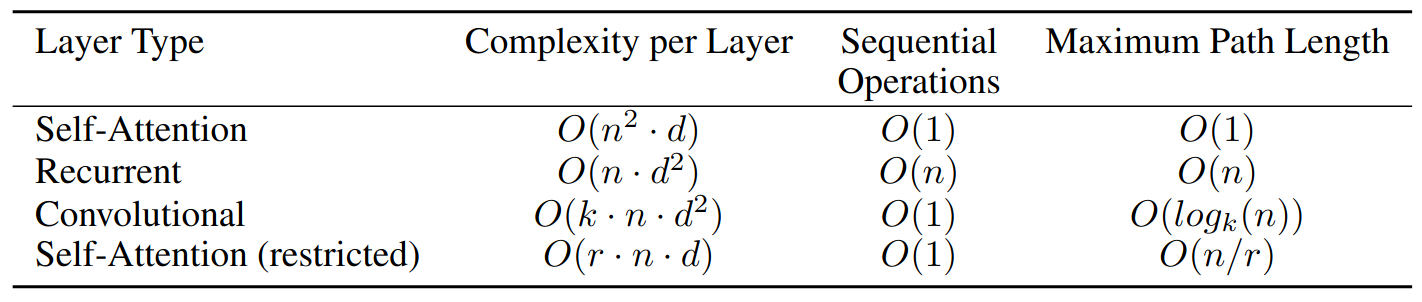
\includegraphics[width=\linewidth]{contents/imgs/transformer_complexity.png}







